\section{Predictions for hadronic final states}
\label{sec:hadronic}

The results presented in Sect.~\ref{sec:inclusive} focused on inclusive observables, where the only acceptance cuts imposed are those of Eq.~(\ref{eq:fiducial}), and where every observable is built from the initial- and final-state leptonic kinematics.
%
We established that the NLO-matched event generators agree with each other and with the analytic \yadism (ZM-VFNS) reference, while \genie displays much larger variations for differential distributions together with an accidental agreement for inclusive cross-sections.
%
We then studied charm production in Sect.~\ref{sec:charm}, inclusive over the rest of the hadronic final state, for which similar qualitative conclusions apply, and where we also found that the various hadronisation models adopted predict rather different yields of the $D$-meson species.

Now we consider observables which depend on modelling of the hadronic final state of the collision.
%
As opposed to the results of Sects.~\ref{sec:inclusive} and~\ref{sec:charm}, for these no analytic reference exists and the comparison is therefore purely between event generators.
%
First, we study the comparison between the different event generators considered for observables sensitive to the hadronic final state and which can be accessed at the FASER$\nu$ emulsion detector.
%
Then, we quantify the dependence of these results on the choice of parton shower and hadronisation algorithms within the same event generator prediction.
%
Finally, we assess the impact of QED radiation in the stability of MC predictions for the same differential distributions.

\paragraph{Hadronic final states for the FASER$\nu$ selection.}
%
Fig.~\ref{fig:hadron-level} displays hadron-level distributions at $E_\ell = 1$~TeV for the FASER$\nu$ selection, Eq.~(\ref{eq:tierE}), nested in the fiducial region Eq.~(\ref{eq:fiducial}), for muon neutral-current and neutrino charged-current DIS.
%
From top to bottom, we show the charged-hadron multiplicity $N_{\rm ch}$, counting the final-state charged hadrons with energies above $1$~GeV within $\tan\theta < 0.5$ of the beam axis, the leading charged hadron's energy $E_{\rm lead}$, the azimuthal separation between the lepton and the summed charged-hadron system $\Delta\phi\lp \ell',\sum h^\pm\rp$, and the outgoing lepton's total momentum $p_{\ell'}$.
%
Note that the latter can be evaluated from the lepton kinematics, but here it also (indirectly) depends on the hadronic final-state modelling in each generator via the FASER$\nu$ selection of Eq.~(\ref{eq:tierE}). 
%
The \powheg, \sherpa and \herwig NLO matched calculations are compared with \genie (GRV98LO), and 
the bottom panels display the ratio to the \powheg predictions.
%
MHOUs, evaluated with \powheg, range between
$+4.3\%/-3.3\%$ for muon DIS and $+0.9\%/-0.7\%$ for neutrino DIS, a similar relative factor as found for the inclusive cross-sections in Sect.~\ref{sec:inclusive}, and mostly flat in the considered kinematical region.

%%%%%%%%%%%%%%%%%%%%%%%%%%%%%%%%%%%%%%
\begin{figure}[!tbp]
  \centering
  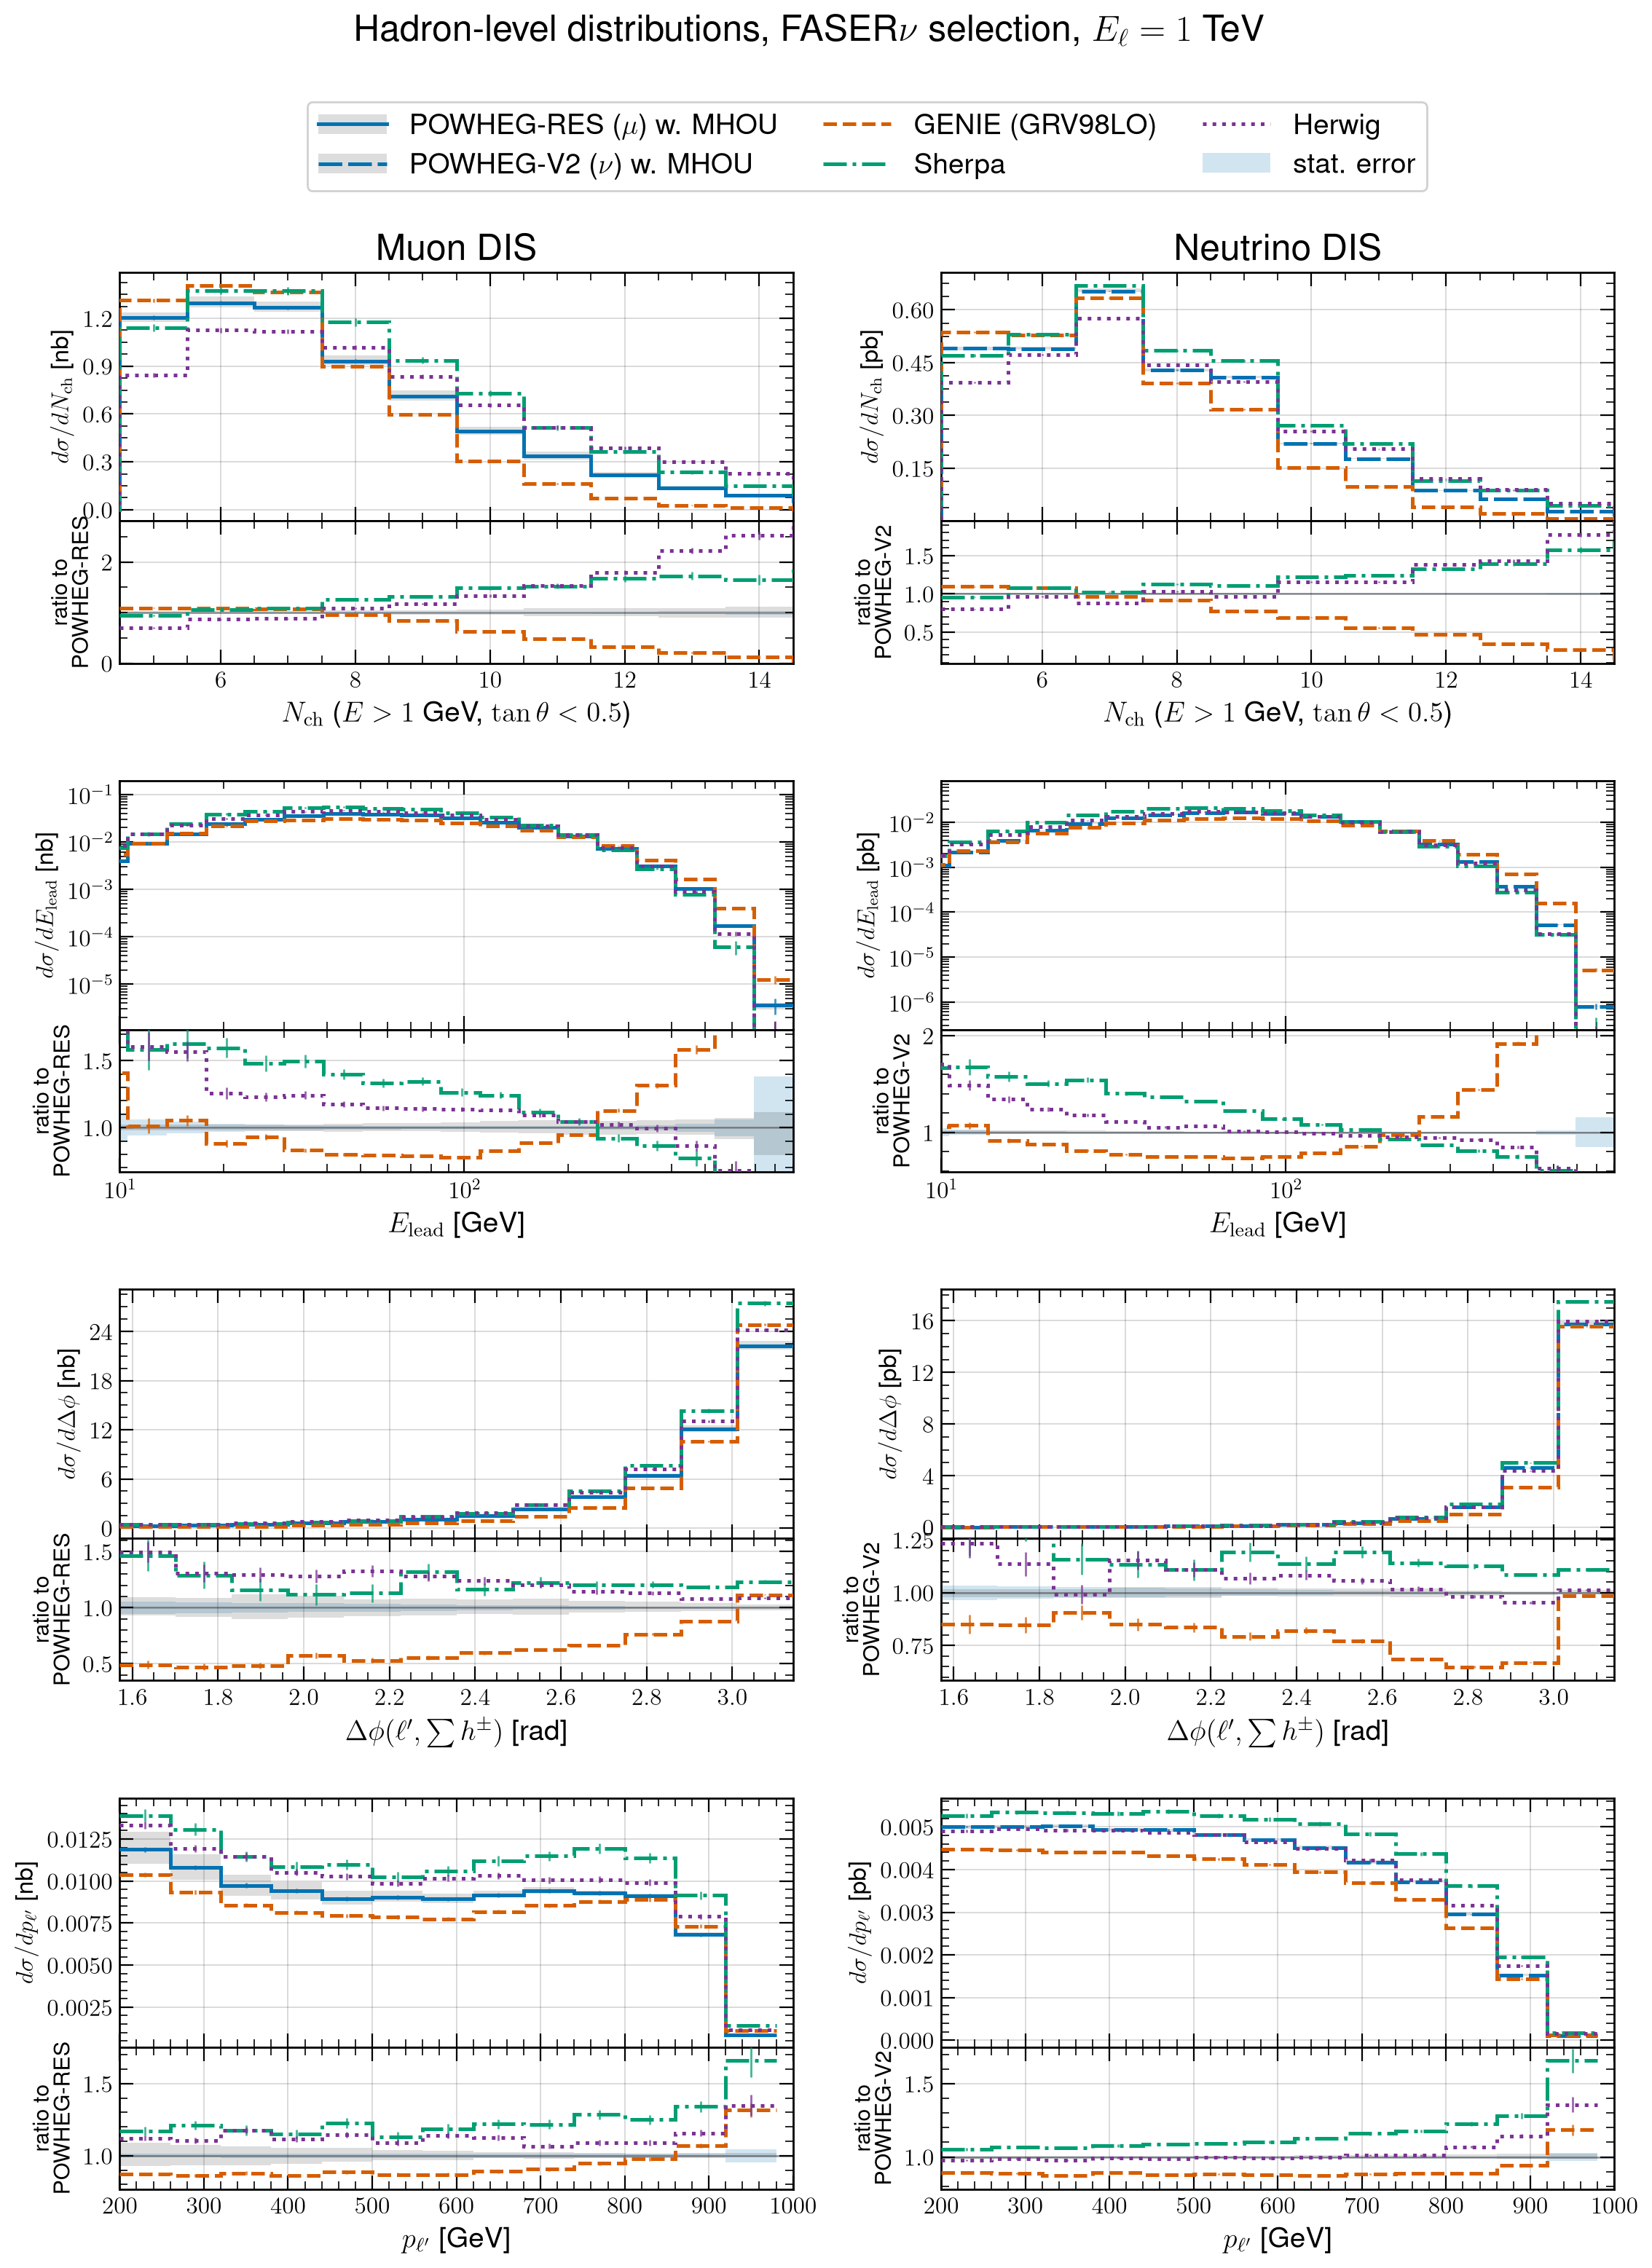
\includegraphics[width=0.94\textwidth]{figures/pp_hadron_level_faser_e.png}
  \caption{Hadron-level distributions per nucleon on tungsten at
    $E_\ell = 1$~TeV for the FASER$\nu$ selection,
    Eq.~(\ref{eq:tierE}), nested in the fiducial region
    Eq.~(\ref{eq:fiducial}), for muon neutral-current (left) and neutrino charged-current
    (right panels) DIS.
    %
    From top to bottom, we show the charged-hadron multiplicity $N_{\rm ch}$
    with energies above $1$~GeV within $\tan\theta < 0.5$ of the beam axis, the leading charged hadron's
    energy $E_{\rm lead}$, the azimuthal separation between the lepton and the summed
    charged-hadron system $\Delta\phi\lp \ell',\sum h^\pm\rp$, and the outgoing lepton's momentum $p_{\ell'}$.
    %
    The \powheg, \sherpa and \herwig NLO matched calculations are compared with \genie (GRV98LO).
    %
    The bottom panels display the ratio to the \powheg predictions, for which the NLO MHOUs are also shown.
   }
  \label{fig:hadron-level}
\end{figure}
%%%%%%%%%%%%%%%%%%%%%%%%%%%%%%%%%

The comparison of Fig.~\ref{fig:hadron-level} indicates that the excellent agreement between NLO-matched generators found for DIS distributions (inclusive and charm production) is lost for observables sensitive to the modelling of the hadronic final state. 
%
For instance, \herwig and \sherpa predict a harder $N_{\rm ch}$ distribution as compared to \powheg; the distributions in $E_{\rm lead}$ are likewise enhanced in \herwig and \sherpa relative to \powheg below 200 GeV and suppressed at higher energies; and also in $\Delta\phi$ and $p_{\ell'}$ the spread between predictions of three calculations at the same nominal perturbative accuracy is large, up to $50\%$ for $\Delta\phi$ and about $30\%$ for $p_{\ell'}$.
%
Significant differences are also found for the \genie predictions: if we compare with \powheg we find a softer large-$N_{\rm ch}$ distribution; suppressed (enhanced) $E_{\rm lead}$ distributions at small (large) values of the leading charged-hadron energy; and a general suppression of the $\Delta \phi$ and $p_{\ell'}$ except possibly at the rightmost bins. 

The mean charged-hadron multiplicity within the FASER$\nu$ acceptance, which is a crucial parameter to identify neutrino and muon DIS events, is $7.7$ for \powhegres, $7.0$ for \genie, $8.2$ for \sherpa and $8.8$ for \herwig in muon DIS, and $7.8$, $7.3$, $8.1$ and $8.2$ respectively in neutrino DIS: that is, as mentioned above, \genie lies below the matched calculations, \sherpa above \powheg and \herwig highest, a spread of up to $26\%$.
%
Concerning the $p_{\ell'}$ predictions, their shape and normalisation agree for the three NLO-matched generators without the FASER$\nu$ cuts (Sect.~\ref{sec:inclusive}), and once the  FASER$\nu$ selection is applied the shapes remain mostly similar but the overall normalisation changes due to the effect of the $N_{\rm ch}$ vertex selection cut.

Two main messages can be drawn from Fig.~\ref{fig:hadron-level}.
%
First, that even at the same formal NLO accuracy differences for hadronic observables remain large, calling for higher-accuracy shower algorithms and tuned fragmentation models for the FASER kinematics.
%
Second, that FASER$\nu$ analyses should assess the stability of their vertex selection cuts with respect to the modelling of distributions such as $N_{\rm ch}$, to avoid biasing their neutrino reconstruction. 

\paragraph{Parton shower and hadronisation dependence.}
%
The comparisons of Fig.~\ref{fig:hadron-level} highlight how differences in the way DIS event generators model the hadronic final state affect predictions for observables relevant for FASER$\nu$.
%
Since the three NLO-matched event generators considered agree for the DIS distributions both for inclusive and for charm production, the differences in Fig.~\ref{fig:hadron-level} must arise from the choice of parton shower algorithm and the treatment of hadronisation in each case.
%
Now we attempt to disentangle some of these effects, by comparing predictions based on the same generator where the parton shower algorithm, and possibly also the hadronisation model, is 
modified keeping all other settings to be the same.

Fig.~\ref{fig:shower-dependence} displays the same final-state hadronic observables as in Fig.~\ref{fig:hadron-level} now with predictions for two of the NLO-matched generators being considered (\powheg and \sherpa) compared for alternative parton shower algorithms.
%
Specifically, for \powheg we compare the results of using \pythia ($p_T$-ordered shower, Lund string hadronisation) and \herwig (angular-ordered shower, cluster model hadronisation), while for \sherpa we compare the default Catani--Seymour shower (CSS) with the Dire shower, keeping in this case the same hadronisation model.
%
Bottom panels are normalised to the \powheg+\pythia prediction, which is taken as the reference, though here the interesting comparison is that between the same event generator run with different shower and/or hadronisation settings. 

%%%%%%%%%%%%%%%%%
\begin{figure}[!tbp]
  \centering
  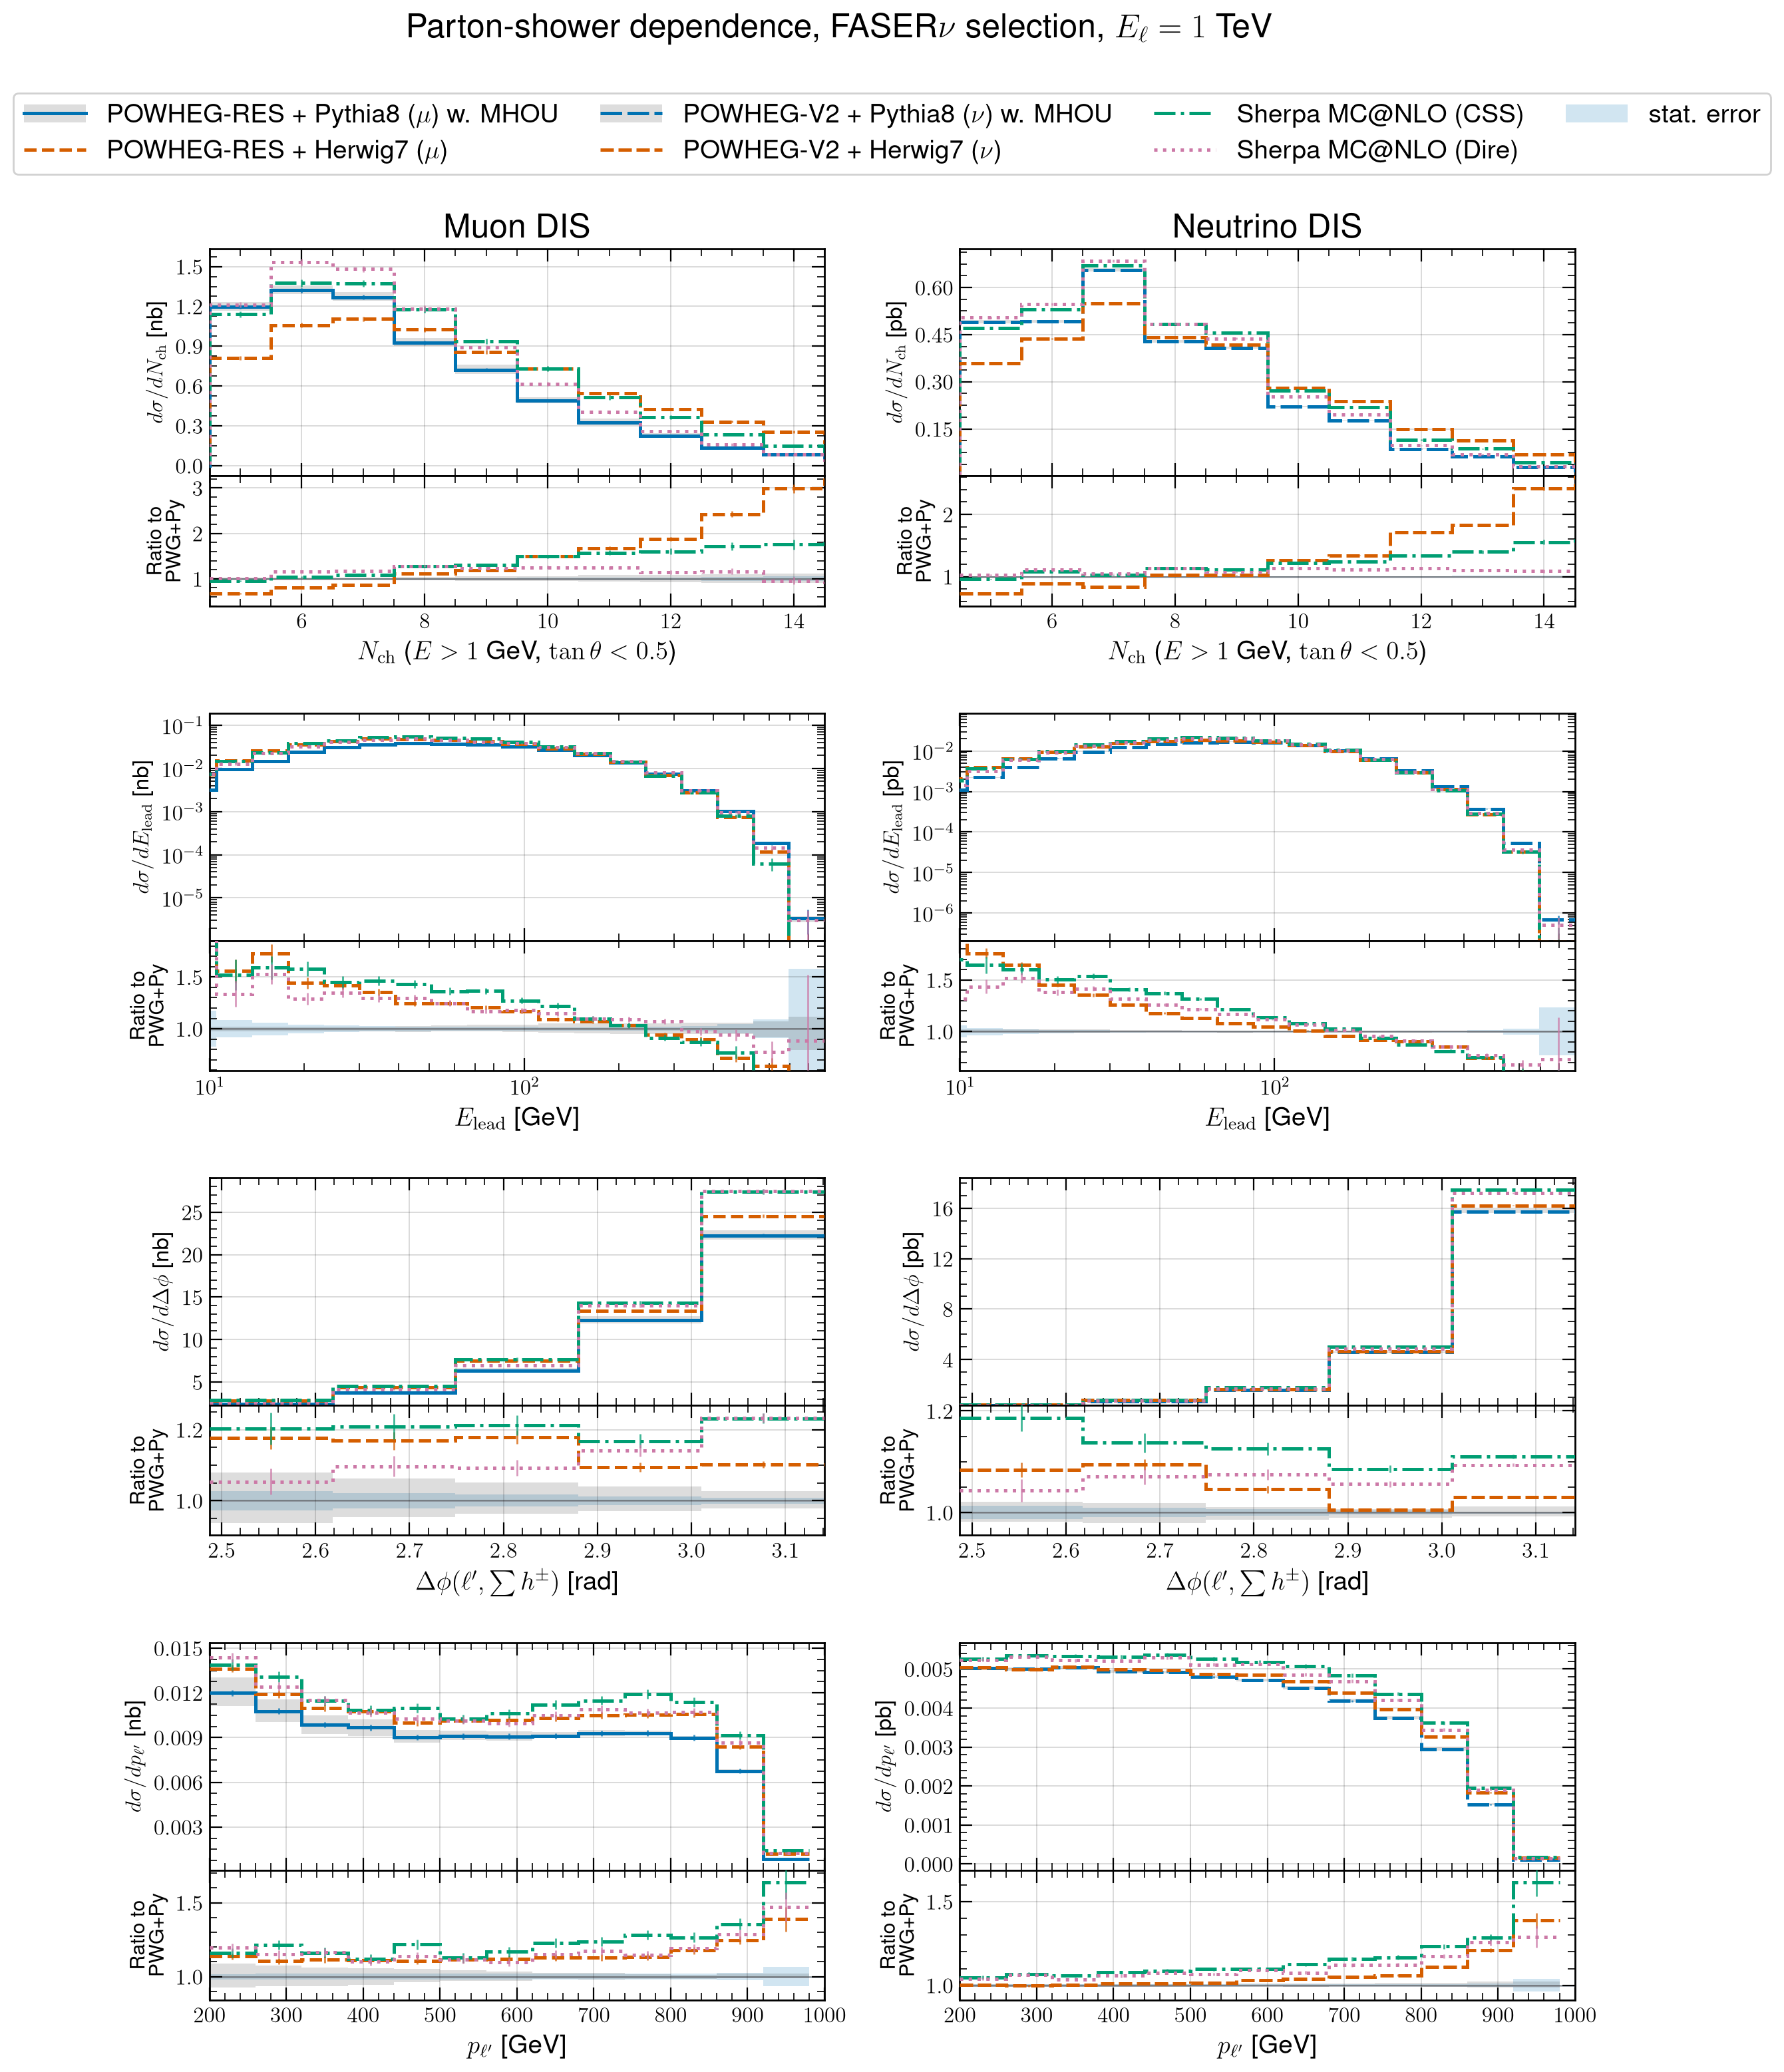
\includegraphics[width=0.99\textwidth]{figures/pp_shower_faser_e.png}
  \caption{
  Same as Fig.~\ref{fig:hadron-level}, now with predictions for two of the NLO-matched generators being considered (\powheg and \sherpa) compared for alternative parton shower algorithms.
  %
  For \powheg we compare the results of using the \pythia and \herwig shower and hadronisation algorithms, while for \sherpa we compare the default CSS with the Dire shower, keeping in this case the same hadronisation model.
  %
  Bottom panels are normalised to the \powheg+\pythia prediction.
  }
  \label{fig:shower-dependence}
\end{figure}
%%%%%%%%%%%%%%%%%

The results of Fig.~\ref{fig:shower-dependence} indicate that $\la N_{\rm ch}\ra$, taken as representative hadronic observable,  moves by $6\%$ ($3\%$) between the two choices of parton shower algorithm available in \sherpa in muon (neutrino) DIS, and by $16\%$ ($10\%$) between the two shower algorithms (\pythia and \herwig) available for \powheg.
%
An uncertainty estimated by switching the shower algorithm within a single event generator is therefore not a complete estimate of the hadronic modelling spread between generators, in particular since parton fragmentation remains a major contribution.
%
Every variation of the  shower algorithm considered here raises the fiducial rates relative to the \powheg reference by up to $21\%$, since the FASER$\nu$ selection demands five charged tracks with four of them narrow, and hence is sensitive to the modelling of the $N_{\rm ch}$ distribution. 
%
As in Fig.~\ref{fig:hadron-level}, the $E_{\rm lead}$ distribution is where the variations separate most: all of them enhance the rate of soft leading hadrons relative to \powheg+ \pythia, by up to about $75\%$ for \powheg+ \herwig between $10$ and $100$~GeV, and suppress it at higher energies, by up to $30$--$40\%$ between $200$ and $600$~GeV.

\paragraph{Impact of QED radiation.}
%
Finally, we consider the impact of QED radiation for differential distributions in muon and neutrino DIS, both for DIS and for final-state hadronic observables.
%
So far, as indicated in Table~\ref{tab:settings}, predictions presented are pure-QCD calculations evaluated at fixed $\alpha_{\rm em}$ in the $G_\mu$ scheme.
%
Here we quantify the role of QED corrections by re-showering the same \powheg events with the QED algorithm of \pythia switched on in stages: final-state radiation (FSR) off the lepton line, initial- and final-state radiation off the lepton line (FSR + ISR), and the full QED shower which also includes radiation off the quark lines.
%
For neutrino DIS there is no ISR off the incoming lepton, and hence the FSR + ISR option does not apply.

%%%%%%%%%%%%%%%%%%%%%%%%%%%%%
\begin{figure}[!tbp]
\centering
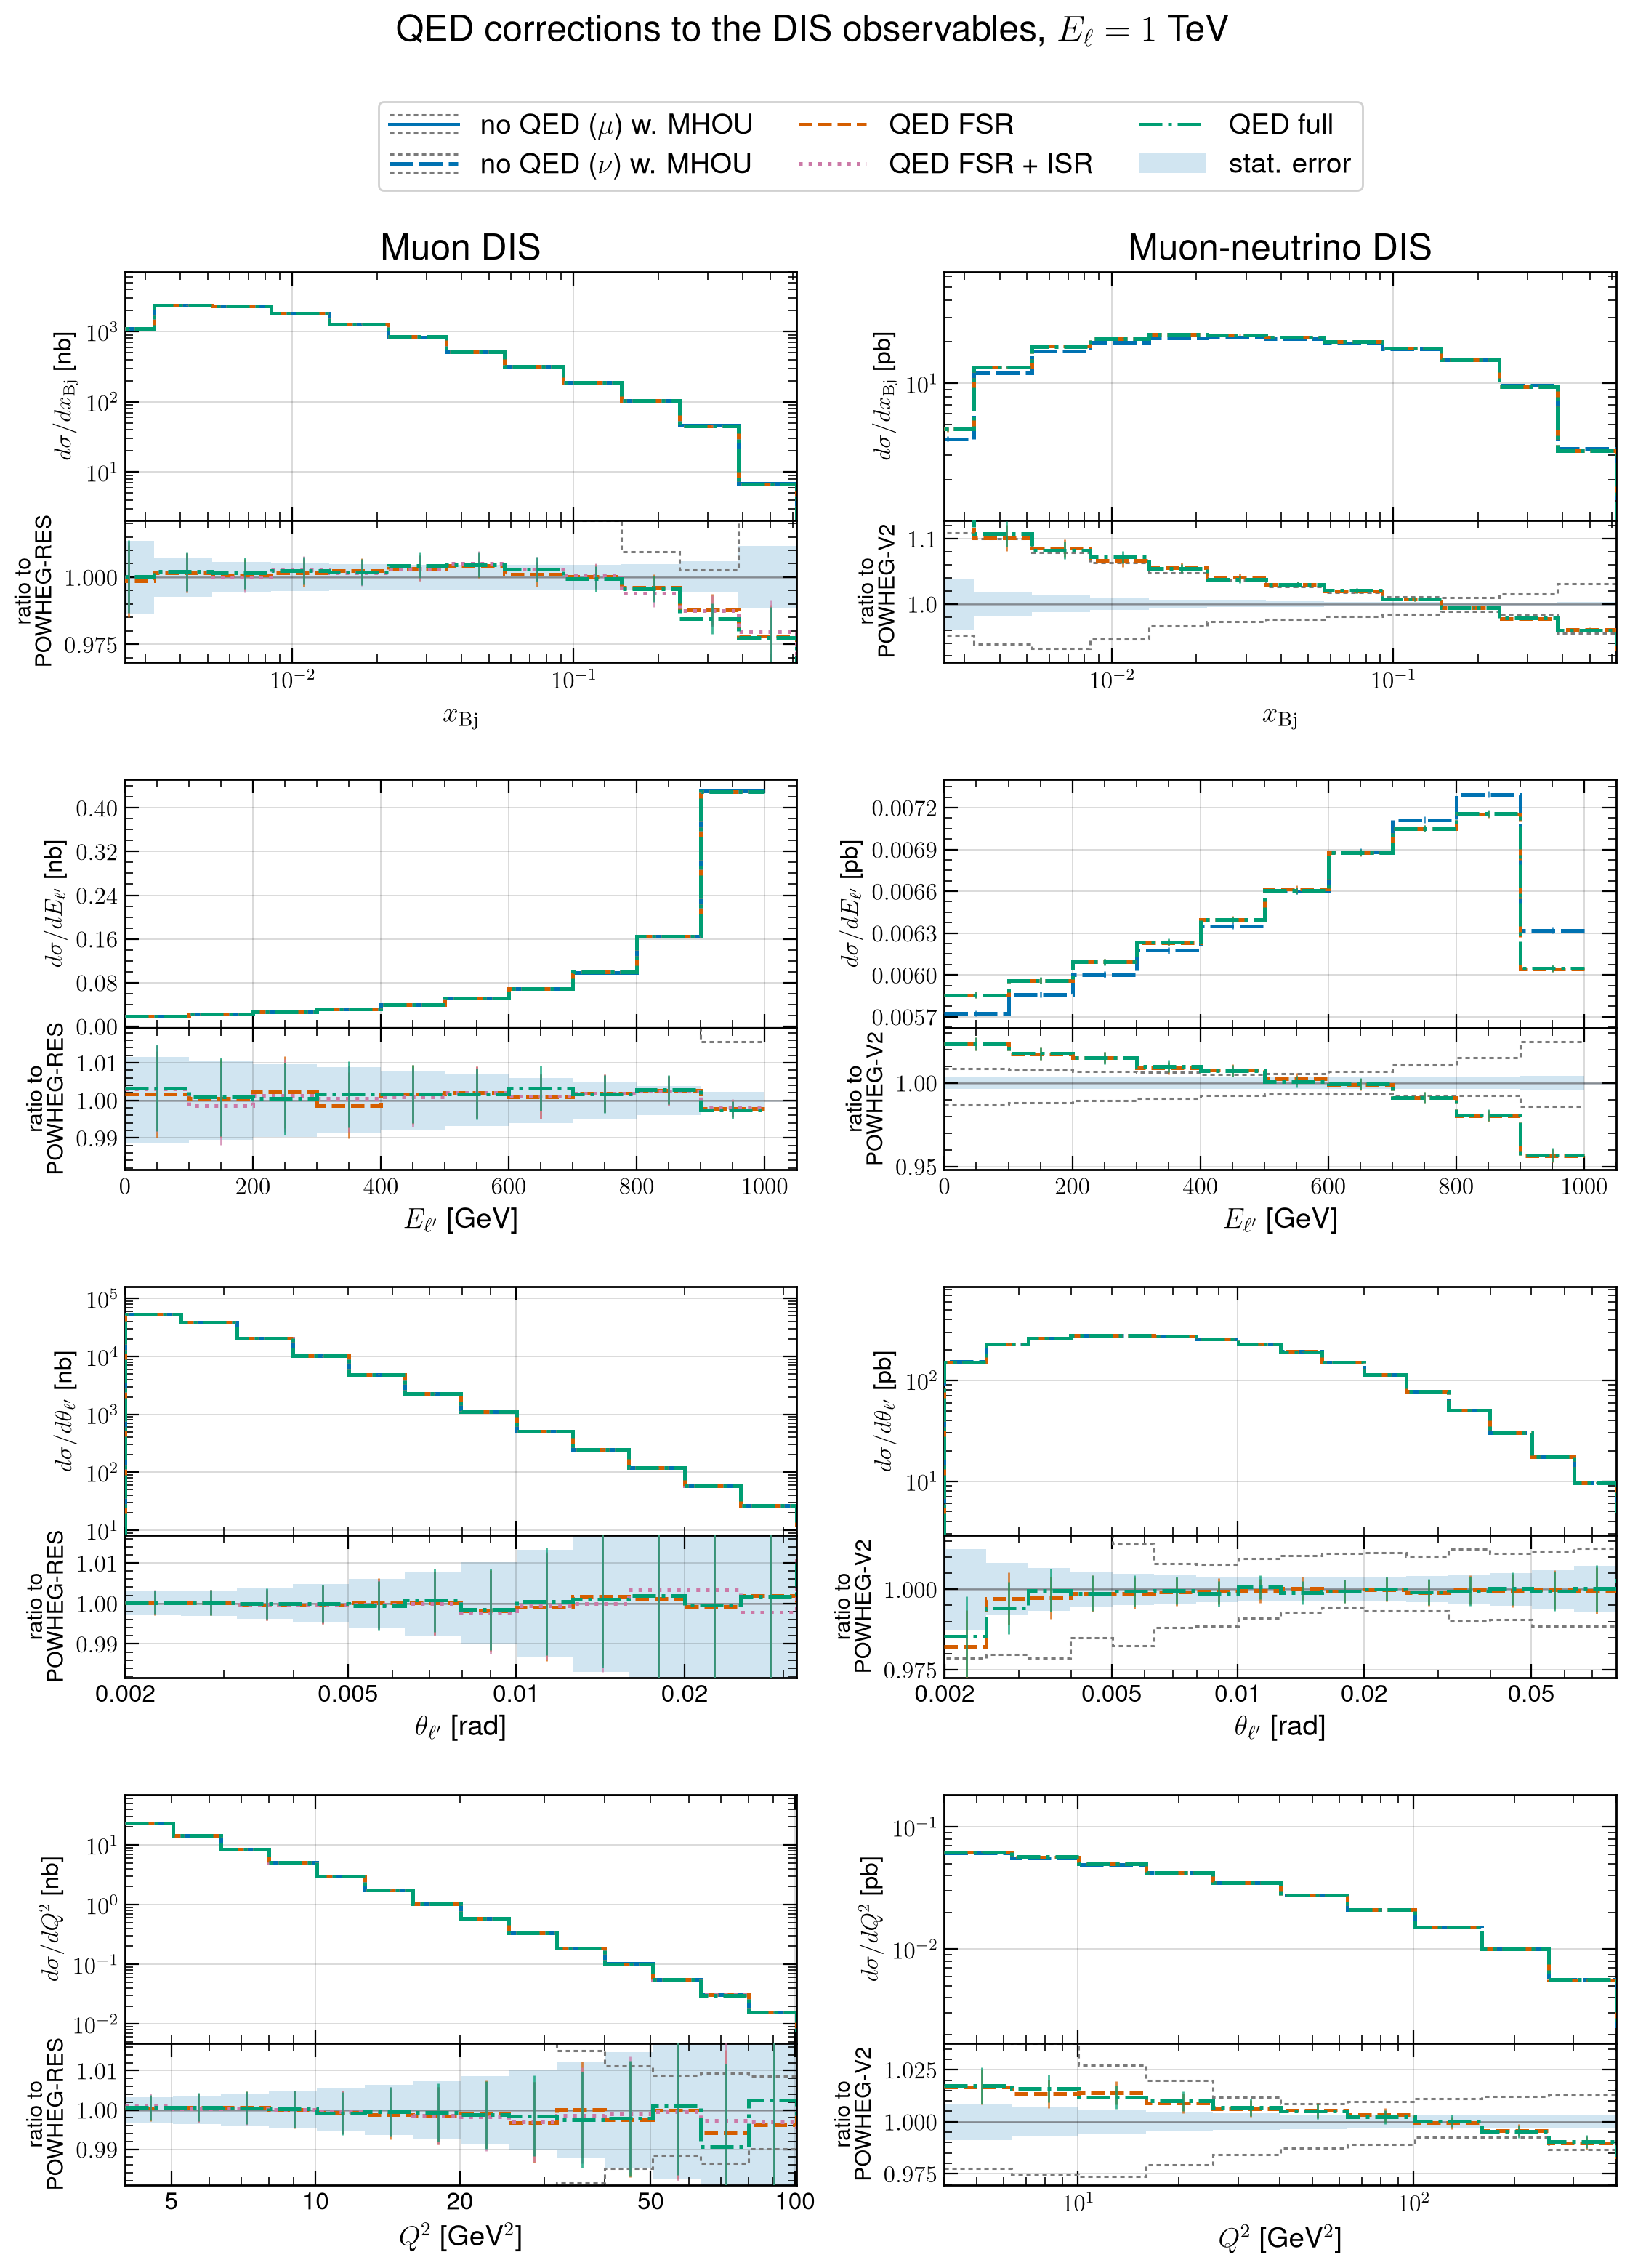
\includegraphics[width=0.90\textwidth]{figures/pp_qed_dis.png}
\caption{The effect of QED radiation on the DIS observables per nucleon on tungsten at $E_\ell = 1$~TeV in the fiducial region Eq.~(\ref{eq:fiducial}) for muon neutral-current (left) and muon-neutrino charged-current (right panels) DIS. 
%
We compare the results of showering a common set of \powheg events with four different options (three for neutrino DIS, where there is no ISR off the incoming lepton): QED radiation off, with final-state radiation only, with initial- and final-state radiation, and then with the full QED shower; the lower panels are ratios to the prediction without QED corrections accounted for.
%
The blue band corresponds to the MC statistical uncertainties, and the dotted lines to the NLO MHOU of the prediction without QED corrections.
%
The effects of QED radiation are known to be larger for electron-neutrino scattering {\it e.g.}~\cite{vanBeekveld:2024ziz}.
}
  \label{fig:qed-dis}
\end{figure}
%%%%%%%%%%%%%%%%%%%%%%%%%%%%%%%

%%%%%%%%%%%%%%%%%%%%%%%%%%%%%%%%%%%%%%
\begin{figure}[!tbp]
  \centering
  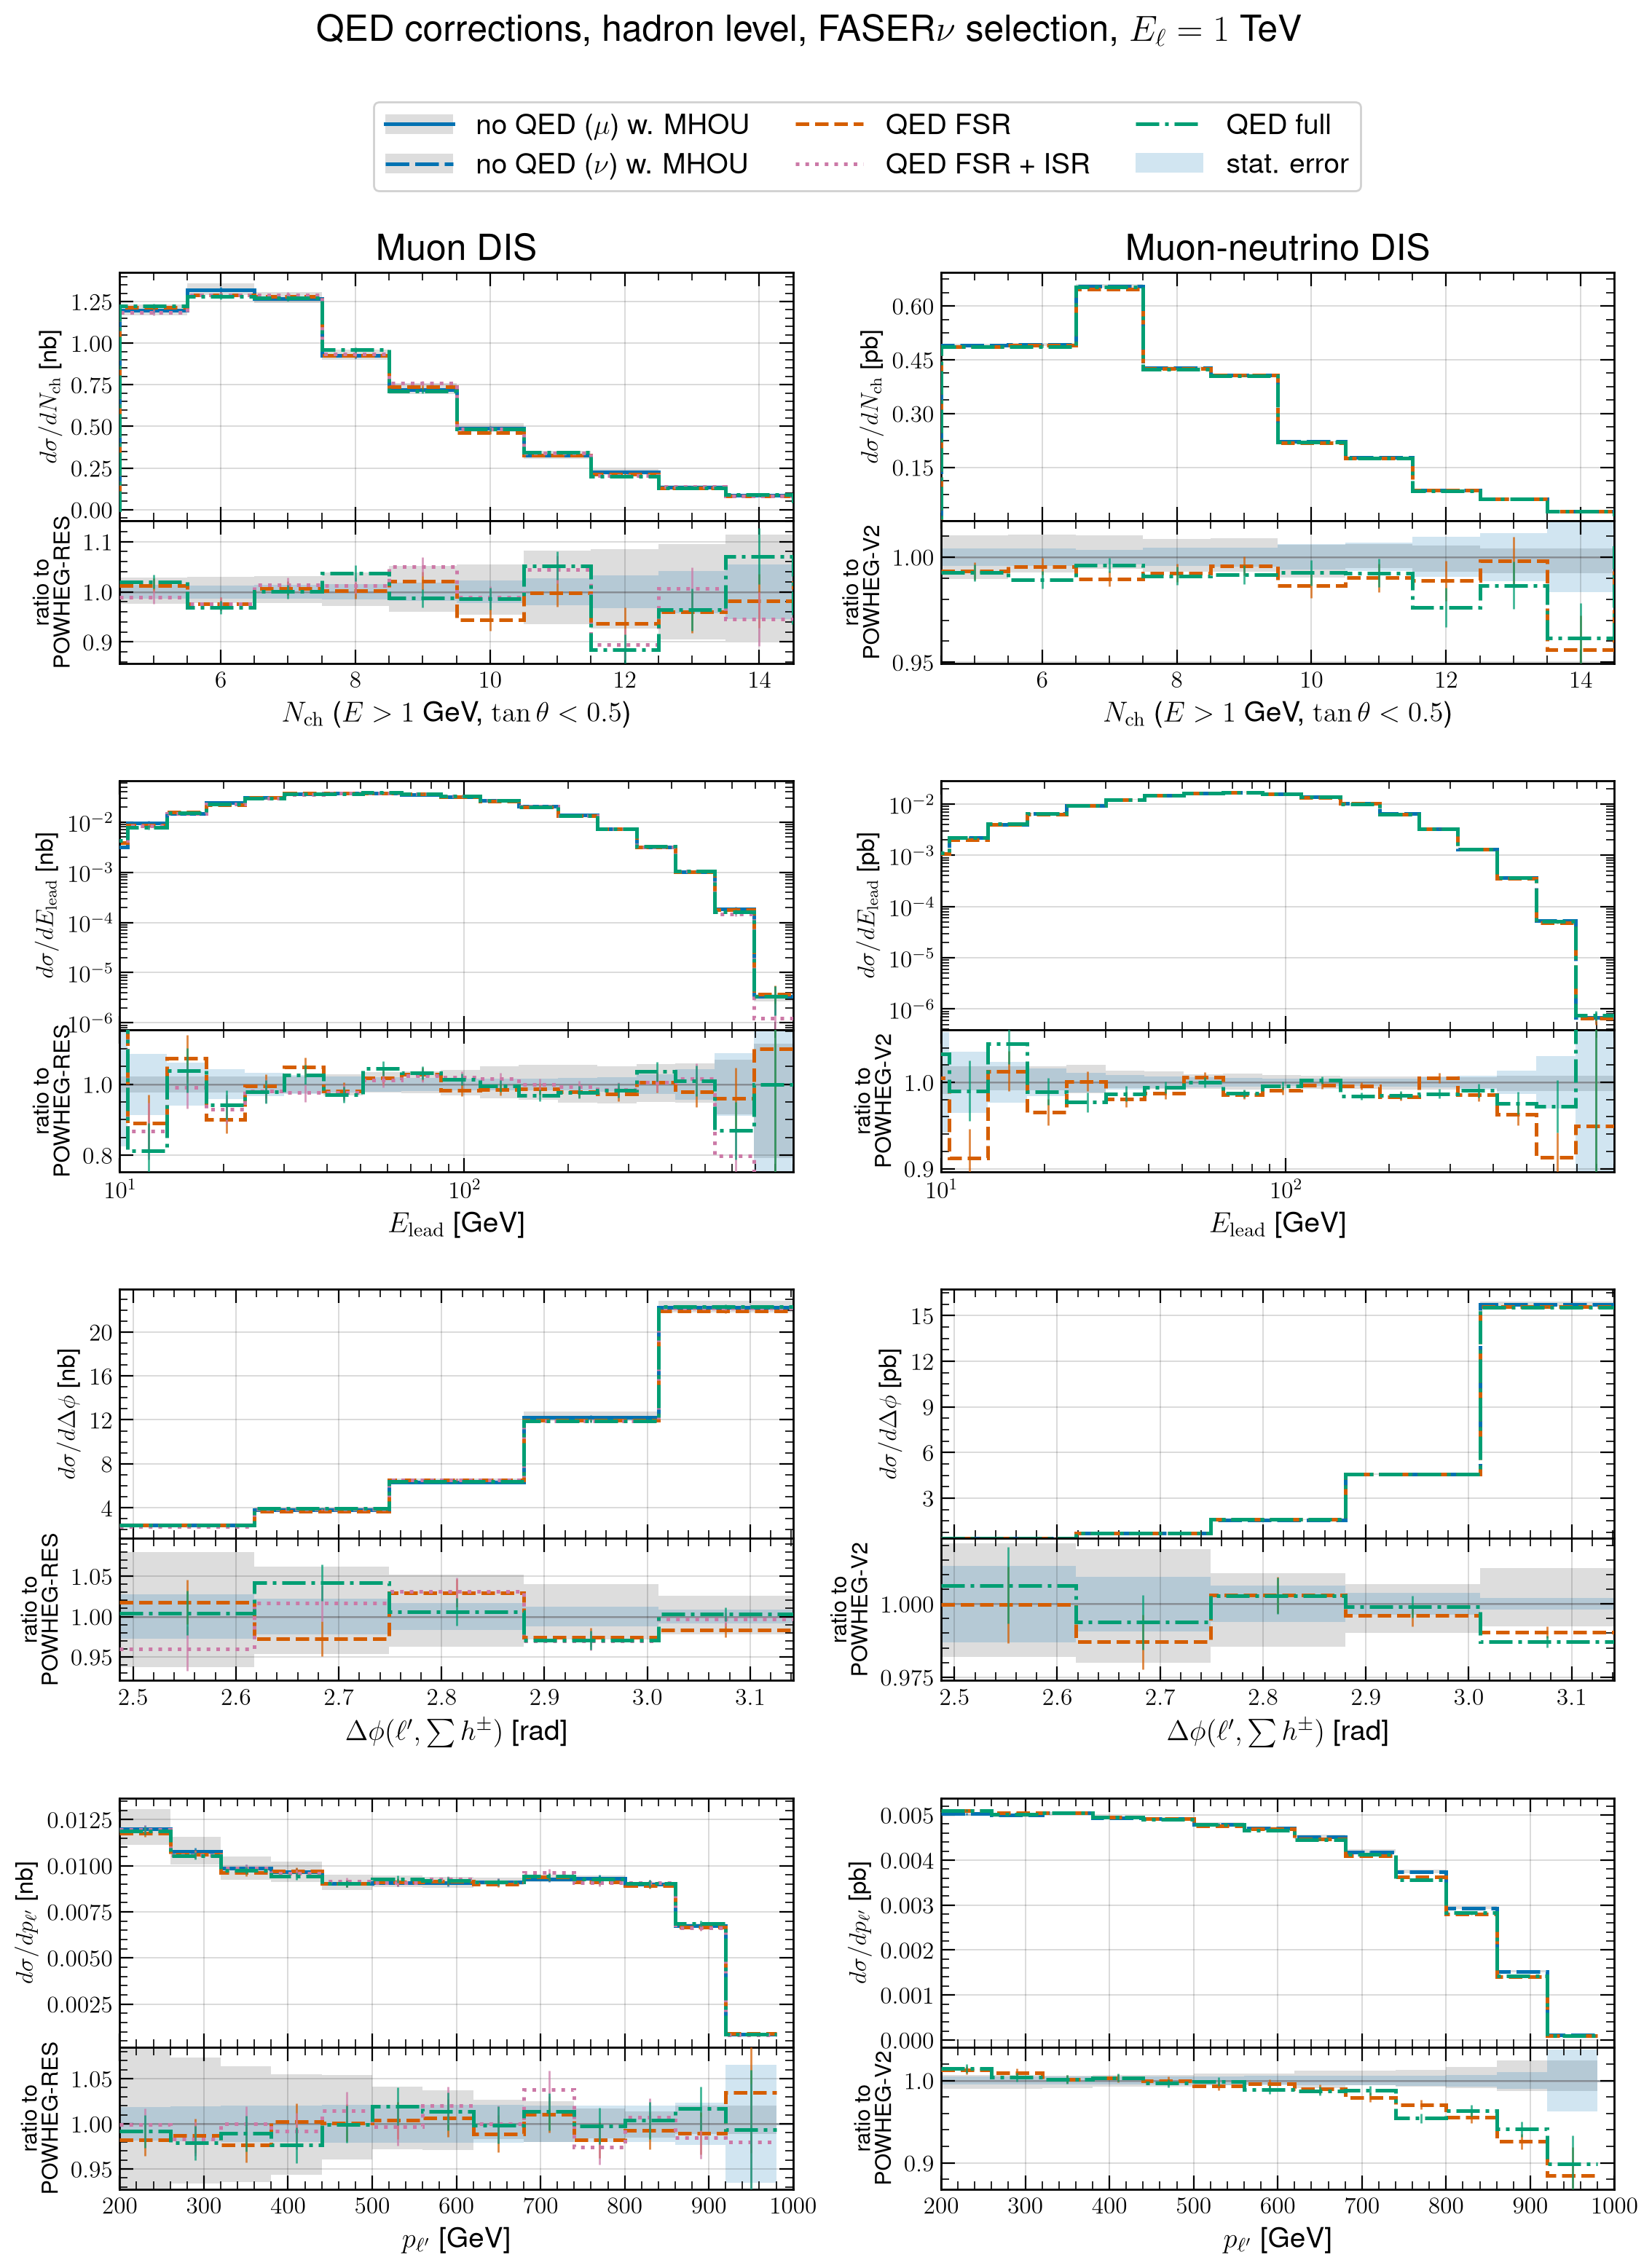
\includegraphics[width=0.99\textwidth]{figures/pp_qed_hadron.png}
  \caption{Same as Fig.~\ref{fig:qed-dis} for the
    hadron-level observables of Fig.~\ref{fig:hadron-level} corresponding to the FASER$\nu$ selection. }
  \label{fig:qed-hadron}
\end{figure}
%%%%%%%%%%%%%%%%%%%%%%%%%%%%%

Fig.~\ref{fig:qed-dis} quantifies the effect of QED radiation on DIS observables at $E_\ell = 1$~TeV in the fiducial region of Eq.~(\ref{eq:fiducial}) for muon neutral-current and muon-neutrino charged-current. 
%
We compare the results of showering a common set of \powheg events with four different options: QED radiation off, with final-state radiation only, with initial- and final-state radiation, and then with the full QED shower; the lower panels are ratios to the prediction without QED corrections accounted for.
%
Note that here it is important to identify the neutrino flavour since QED radiation effects vary with the charged-lepton mass, and in particular they are larger for electron-neutrino than for muon-neutrino scattering~\cite{vanBeekveld:2024ziz}.

Integrated over the fiducial region, QED radiation effects turn out to be negligible (below the per-mille level for both currents).  
%
Differentially, the NC and CC distributions behave differently due to the charge of the incoming lepton in each case.
%
In neutrino DIS, final-state radiation softens the scattered muon systematically: $E_{\ell'}$ increases by a few per cent below $E_{\ell'}\sim 600$ GeV, while at higher energies the spectrum decreases by up to $4$--$5\%$.
%
Since $x_{\rm Bj}$ and $Q^2$ are reconstructed from the scattered lepton kinematics, they shift accordingly.
%
These migrations take place inside the fiducial region explaining why the integrated effect vanishes.
%
In muon DIS the same distributions move by less than $1\%$: the muon is charged both in the initial and in the final state, so the radiation forms a dipole between the two lepton legs and its effect on the reconstructed kinematics largely cancels.
%
Radiation off the quark line, measured from the difference between the full calculation and the partial FSR + ISR one, is not resolved in either current.
%
For muon DIS, and for $\theta_{\ell'}$ and $Q^2$ in neutrino DIS, the effects of QED radiation are smaller than the NLO MHOU; for $x_{\rm Bj}$ and $E_{\ell'}$ in neutrino DIS they exceed it, reaching about $10\%$ at the smallest $x_{\rm Bj}$ and $4\%$ at the largest $E_{\ell'}$.

Fig.~\ref{fig:qed-hadron} presents the corresponding comparison for the hadronic observables of Fig.~\ref{fig:hadron-level} within the FASER$\nu$ selection.
%
In neutrino DIS, since the selection cuts on the lepton momentum, the softening of the scattered muon costs the selected rate around $1\%$ and removes $4$--$6\%$ of the events with $p_{\ell'}>800$ GeV.
%
Beyond this overall selection cut, the hadronic observables do not move.
%
As for the DIS observables, for muon DIS these QED effects are smaller than  other sources of theory uncertainty.

Crucially, we emphasise that the comparisons presented in this section provide a shower-level estimate of QED effects in lepton-nucleon DIS but are not the complete picture.
%
A full calculation involves both the full electroweak virtual corrections, evaluated in a consistent electroweak scheme, as well as photon-initiated contributions to lepton-nucleon scattering~\cite{Manohar:2016nzj,Bertone:2017bme,Manohar:2017eqh,Cridge:2021pxm,NNPDF:2024djq}.
%
The conclusion of this study is nevertheless robust: for the FASER fiducial kinematics, QED radiation is a sub-per-cent effect on the inclusive rates, and its only visible signature is the softening of the scattered-lepton spectrum in charged-current scattering, which shifts the reconstructed $x_{\rm Bj}$ and $E_{\ell'}$ distributions by several per cent, beyond the NLO MHOU.
%
The latter finding is however restricted to muon-neutrino DIS, and larger effects may be expected for electron-neutrino scattering.
